\documentclass[11pt]{article}
\usepackage[a4paper, margin=2cm]{geometry}
\usepackage[utf8]{inputenc}
\usepackage{babel}
\usepackage[spanish]{layout}
\usepackage[article]{ragged2e}
\usepackage{textcomp}
\usepackage{amsmath}
\usepackage{amssymb}
\usepackage{amsfonts}
\usepackage{proof}
\usepackage{enumerate}
\usepackage{graphicx}
\usepackage{multirow}
\usepackage{caption}
\usepackage{subcaption}

\setlength{\parindent}{0pt}

\title{
    Entregas 8 y 9 \\
    \large Sistemas Operativos II}
\author{Mellino, Natalia \and Farizano, Juan Ignacio}

\date{}

\begin{document}
\maketitle

\noindent\rule{\textwidth}{1pt}

\section*{Ejercicio 1}

\begin{figure}[h!]
    \begin{center}
      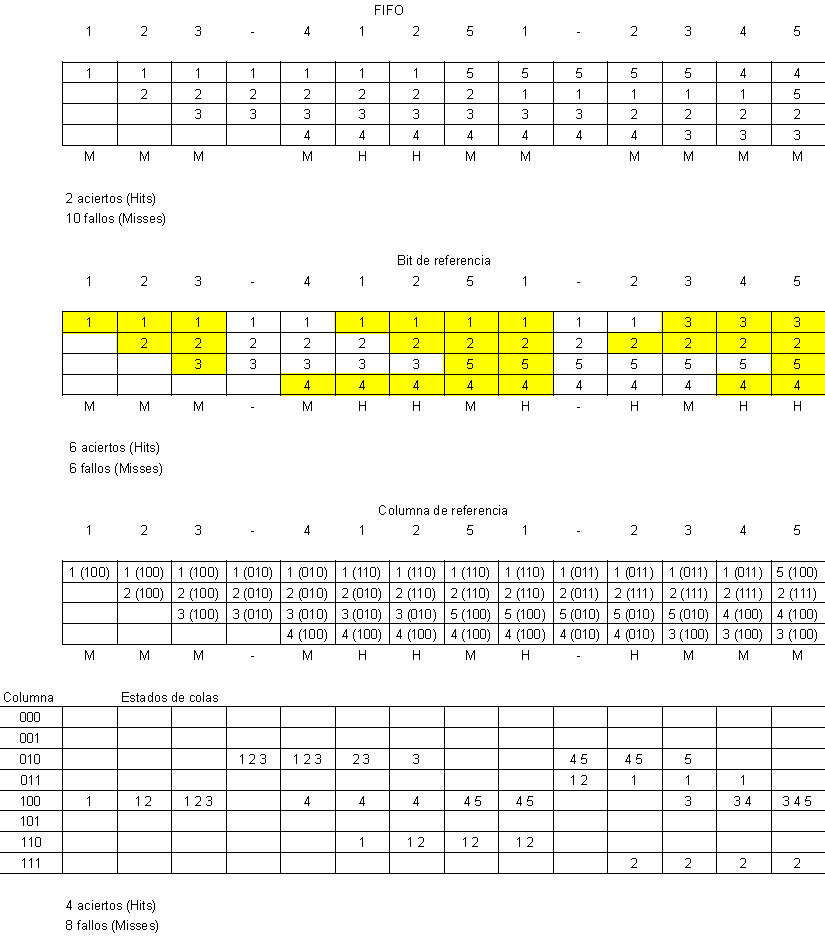
\includegraphics[width=0.85\linewidth]{Paginación.pdf}
    \end{center}
  \end{figure}

\section*{Ejercicio 2}

El conjunto activo de un proceso es el conjunto de páginas sobre los que está
iterando en un momento dado, mientras que el mínimo de marcos es el número
mínimo de marcos que un proceso debe tener asignado. Cada vez que un proceso
genera un fallo de página se le asigna uno de los marcos disponibles. Según cada 
arquitectura, una instrucción puede provocar más de un fallo de página, por lo
tanto es importante tener un número mínimo de marcos adecuados.

El parámetro específico de cada proceso es el conjunto activo (que indica el
conjunto de páginas en el que el proceso tiene su atención y este lo puede
cambiar según necesite), ya que este depende exclusivamente del proceso,
en cambio, el mínimo de marcos depende exclusivamente de la arquitectura.
Todas las arquitecturas proporcionan instrucciones de referencia directa a
memoria que permiten especificar una dirección de memoria para leer o escribir.
Esto indica que todas las arquitecturas requerirán que cada proceso tenga
\textbf{al menos} dos marcos asignados.

\section*{Ejercicio 3}

Ventajas:

\begin{itemize}
    \item Disminuyen los fallos de página. Lo cual disminuye la probabilidad de
          que se produzca \emph{hiperpaginación}.
    \item Los programas se encuentran con una menor latencia al acceder a una
          página por primera vez.
    \item El manejo de memoria con reemplazo de páginas es menos complejo.
\end{itemize}

Desventajas:

\begin{itemize}
    \item Los programas se encuentran con un mayor retraso al inicializar
          ya que es necesario traer más información del disco a la memoria principal.
    \item Los cambios de contexto suelen ser más lentos al tener menos memoria,
          ya que al contar con menos espacio se tienen menos procesos cargados
          disponibles para correr.
\end{itemize}

\end{document}